\newpage
\section{Projektowanie}		%3
%Narysować graf, UML, diagram klas, schemat działania algorytmu

\subsection{Narzędzia i technologie}

W projekcie wykorzystano następujące narzędzia i technologie:

\begin{itemize}
  \item \textbf{Język programowania:} C++.
  \item \textbf{Kompilator:} GCC (GNU Compiler Collection) dla systemów Linux oraz MINGW-w64 dla systemu Windows.
  \item \textbf{System budowania:} CMake z użyciem Ninja jako generatora systemu budowania.
  \item \textbf{Dokumentacja:} Narzędzie \texttt{Doxygen} do generowania dokumentacji technicznej oraz szablon \LaTeX{} dostosowany przez mgr inż. Dawida Kotlarskiego.
  \item \textbf{Kontrola wersji:} Git oraz platforma GitHub.
  \item \textbf{Git Hooks:} Lefthook do automatyzacji zadań związanych z Git.
  \item \textbf{Continuous Integration:} GitHub Actions do automatyzacji testów i budowy projektu.
  \item \textbf{Walidacja commitów:} Narzędzie \texttt{Commitlint} do sprawdzania wiadomości commitów zgodnie z konwencją Conventional Commits.
\end{itemize}

\subsection{Ustawienia kompilatora}

Projekt korzysta z systemu CMake, który umożliwia konfigurację i zarządzanie ustawieniami kompilatora dla różnych platform. Ustawienia są dostosowane do pracy z:

\begin{itemize}
  \item \textbf{Windows:} MINGW-w64 z MSYS2 jako środowiskiem terminalowym.
  \item \textbf{Linux:} GCC, który jest standardowym kompilatorem na większości dystrybucji systemu Linux.
\end{itemize}

Dzięki zastosowaniu CMake projekt jest w stanie automatycznie generować odpowiednie pliki Makefile dla Ninja, co umożliwia szybkie i efektywne budowanie aplikacji.

\subsection{Schemat działania programu}

Na rysunku \textbf{3.1} przedstawiono diagram UML klas, który ilustruje strukturę i relacje pomiędzy klasami w projekcie.

\begin{figure}[!htb]
  \begin{center}
    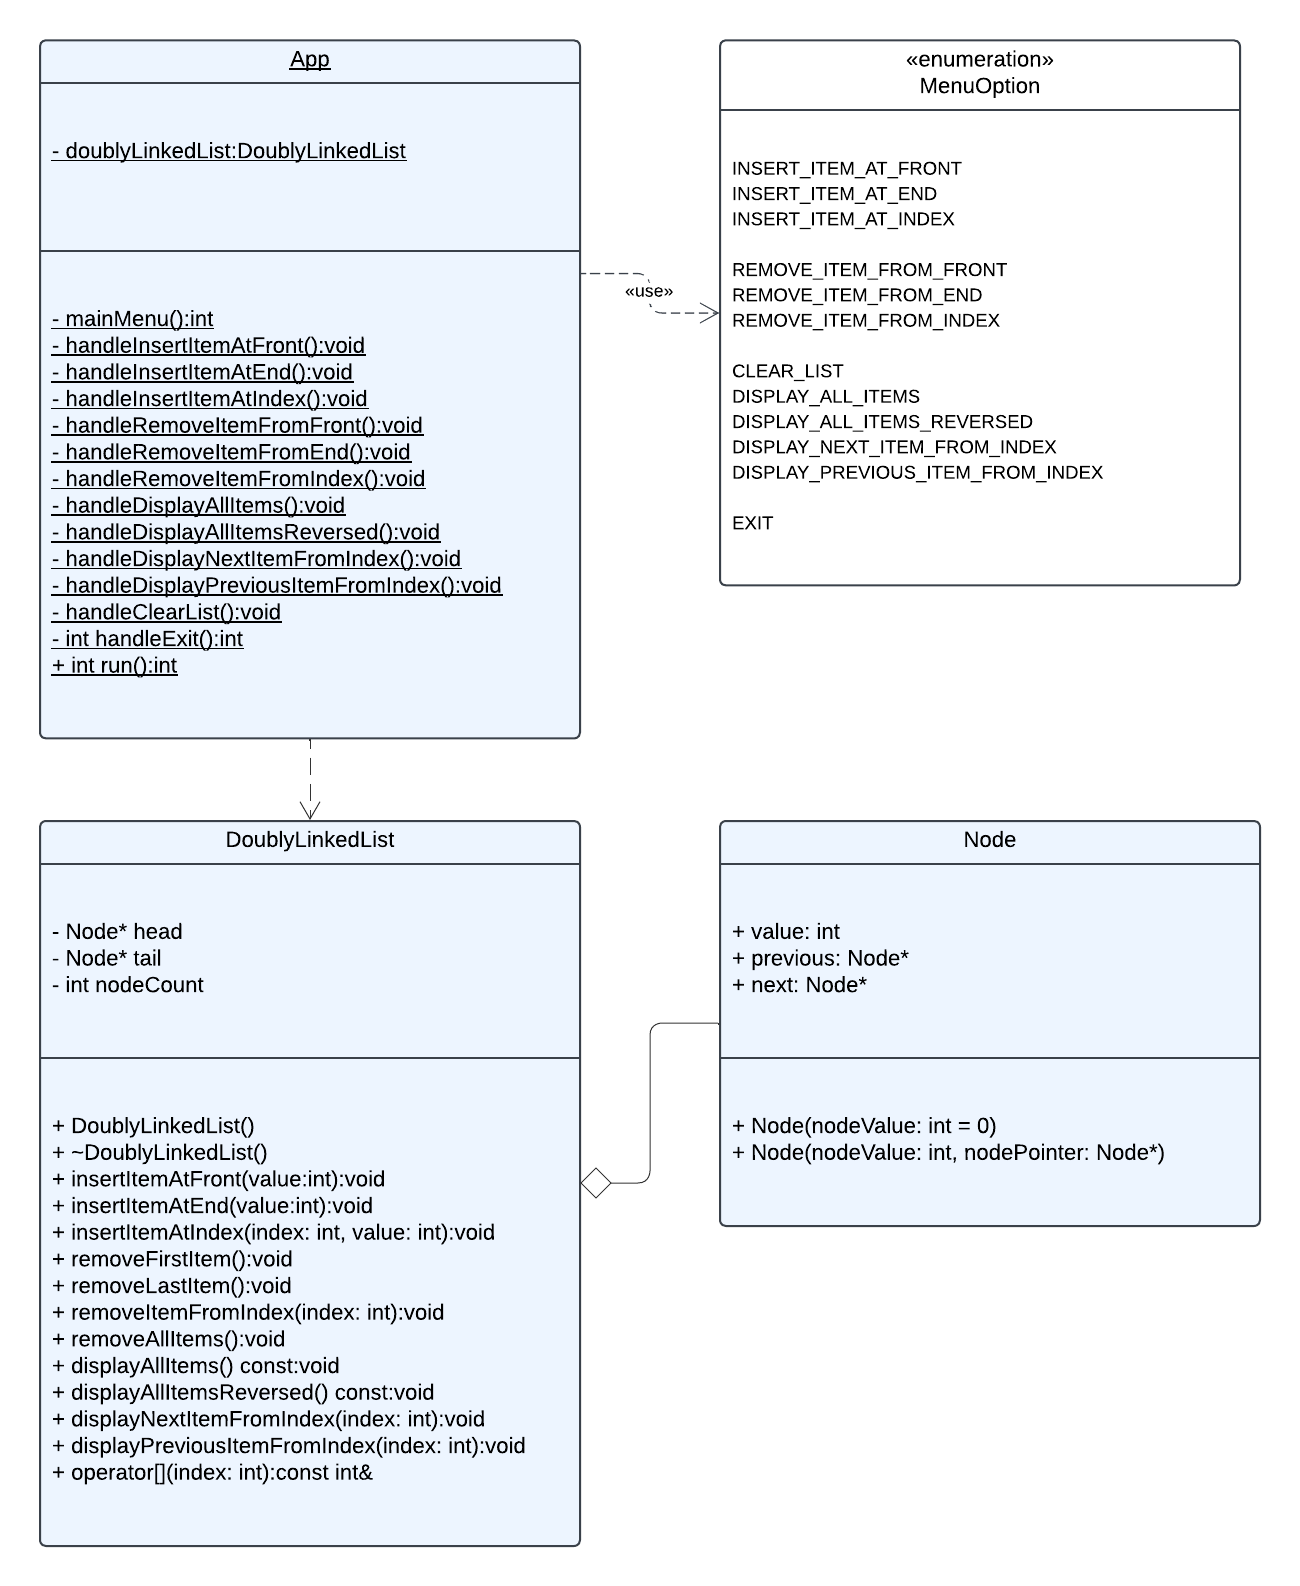
\includegraphics[width=\textwidth]{rys/diagram_UML.png}
    \caption{Diagram UML klas dla projektu}\label{fig:uml_diagram}
  \end{center}
\end{figure}

\subsection{Użycie narzędzi}

Na potrzeby tego i przyszłych projektów o podobnym charakterze
został utworzony szablon repozytorium na platformie GitHub.
Znajduje jest ono pod adresem: \url{https://github.com/Me-Phew/programowanie-zaawansowane-template}\cite{GitHubProjectTemplate} (Dostęp: 24.10.2024r.).
Zawiera następujące funkcjonalności:

\begin{itemize}
  \item \textbf{Generator systemu budowania:} CMake do zarządzania konfiguracją projektu.
  \item \textbf{Kompleksowa konfiguracja dla GCC (MINGW-w64) oraz Linux.}
  \item \textbf{Automatyzacja budowy projektu:} Ninja jako system budowania.
  \item \textbf{Dokumentacja:} Generowana automatycznie z użyciem Doxygen oraz szablonu LaTeX.
  \item \textbf{Zarządzanie tematami:} Temat Doxygen Awesome z kolorami inspirowanymi stroną Nuxt.
  \item \textbf{Git Hooks:} Lefthook do automatyzacji i walidacji wiadomości commitów.
  \item \textbf{Continous Integration:} GitHub Actions do automatyzacji procesów budowy i testowania.
  \item \textbf{Generowanie strony dokumentacji automatycznej:} GitHub Pages.
  \item \textbf{Tworzenie wydań:} Zawierające pliki wykonywalne dla systemów Windows i Linux oraz pliki dokumentacji.
\end{itemize}

\newpage

\subsection{Przykładowa konfiguracja CMake}

Przykładowa konfiguracja pliku \texttt{Zawartość pliku CMakeLists.txt} dla projektu została przedstawiona
na listingu \textbf{1}

\begin{lstlisting}[caption=CMakeLists.txt, label={lst:listing-CMakeLists.txt}, language=C++]
cmake_minimum_required(VERSION 3.10)

project(DoublyLinkedList)

include_directories(src/app src/doubly_linked_list)

set(SOURCES src/app/app.cpp src/doubly_linked_list/doubly_linked_list.cpp src/main.cpp)

add_executable(DoublyLinkedList ${SOURCES})

# Compile with all warnings, treat warnings as errors
if (MSVC)
		add_compile_options(/W4 /WX)
else()
		add_compile_options(-Wall -Wextra -pedantic -Werror)
endif()
\end{lstlisting}

Powyższa konfiguracja definiuje minimalną wersję CMake, ustawia standard C++ oraz określa pliki źródłowe projektu.
